\section{Procedure}
\subsection{Falling Sphere 


\begin{figure}
    \begin{minipage}{.3\textwidth}
        \centering
        \vspace{4.mm}
        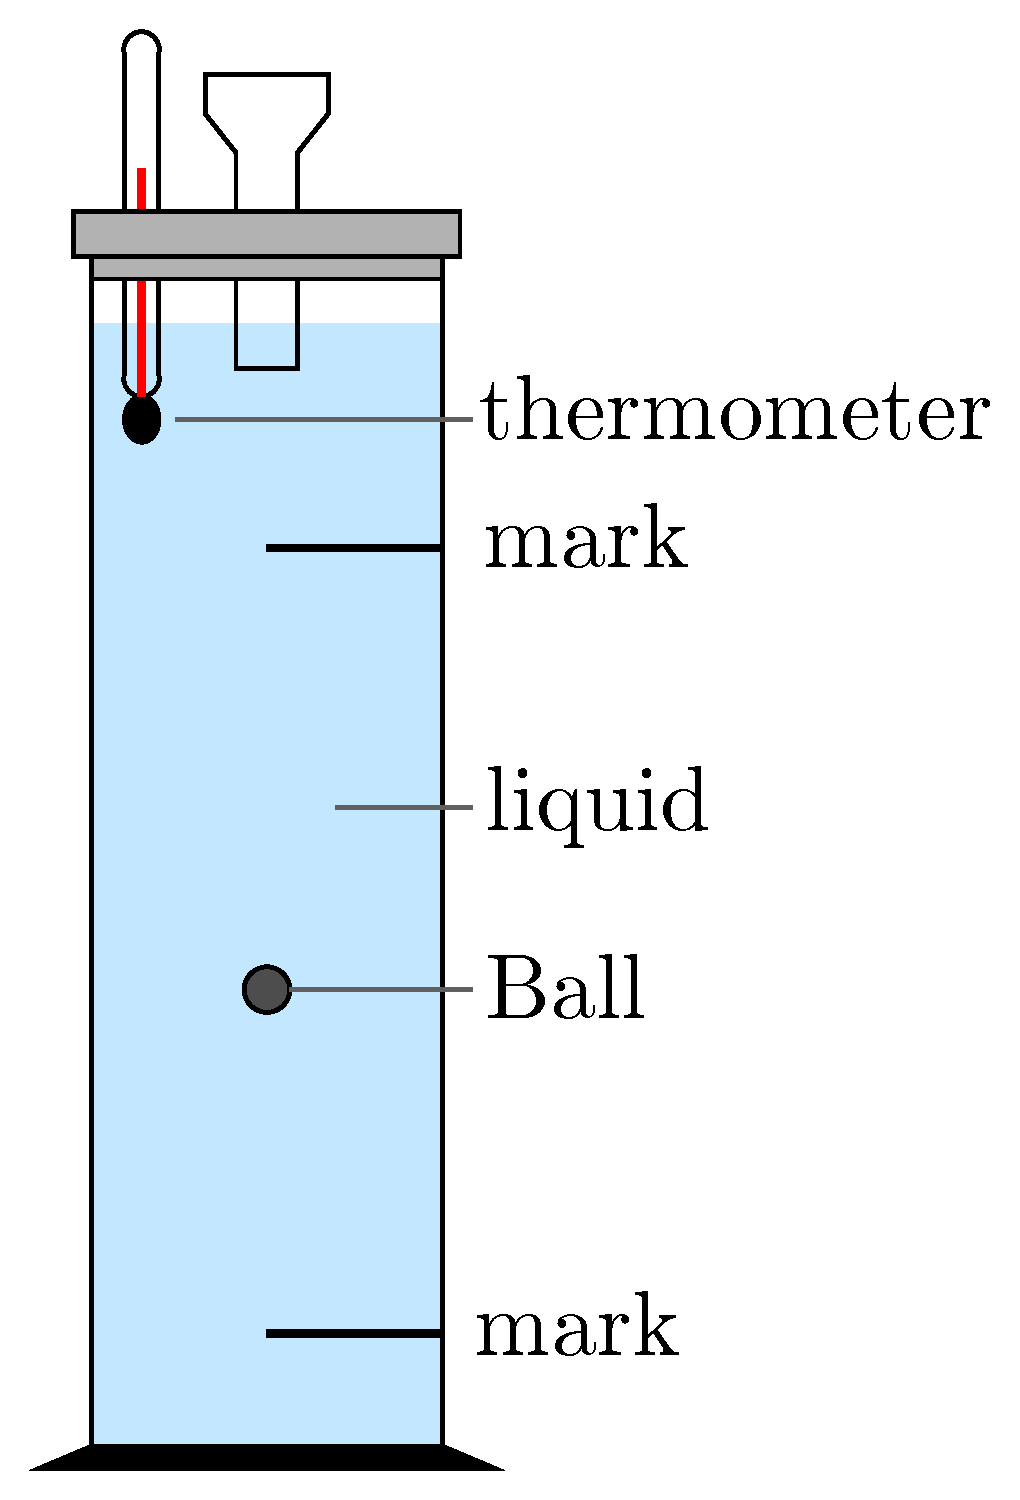
\includegraphics[scale=.25]{Bilder/kugelfall.pdf}
        \vspace{4.mm}
        \caption{falling sphere viscometer}
    \end{minipage}
    \hspace{5mm}
    \begin{minipage}{.3\textwidth}
    \centering
    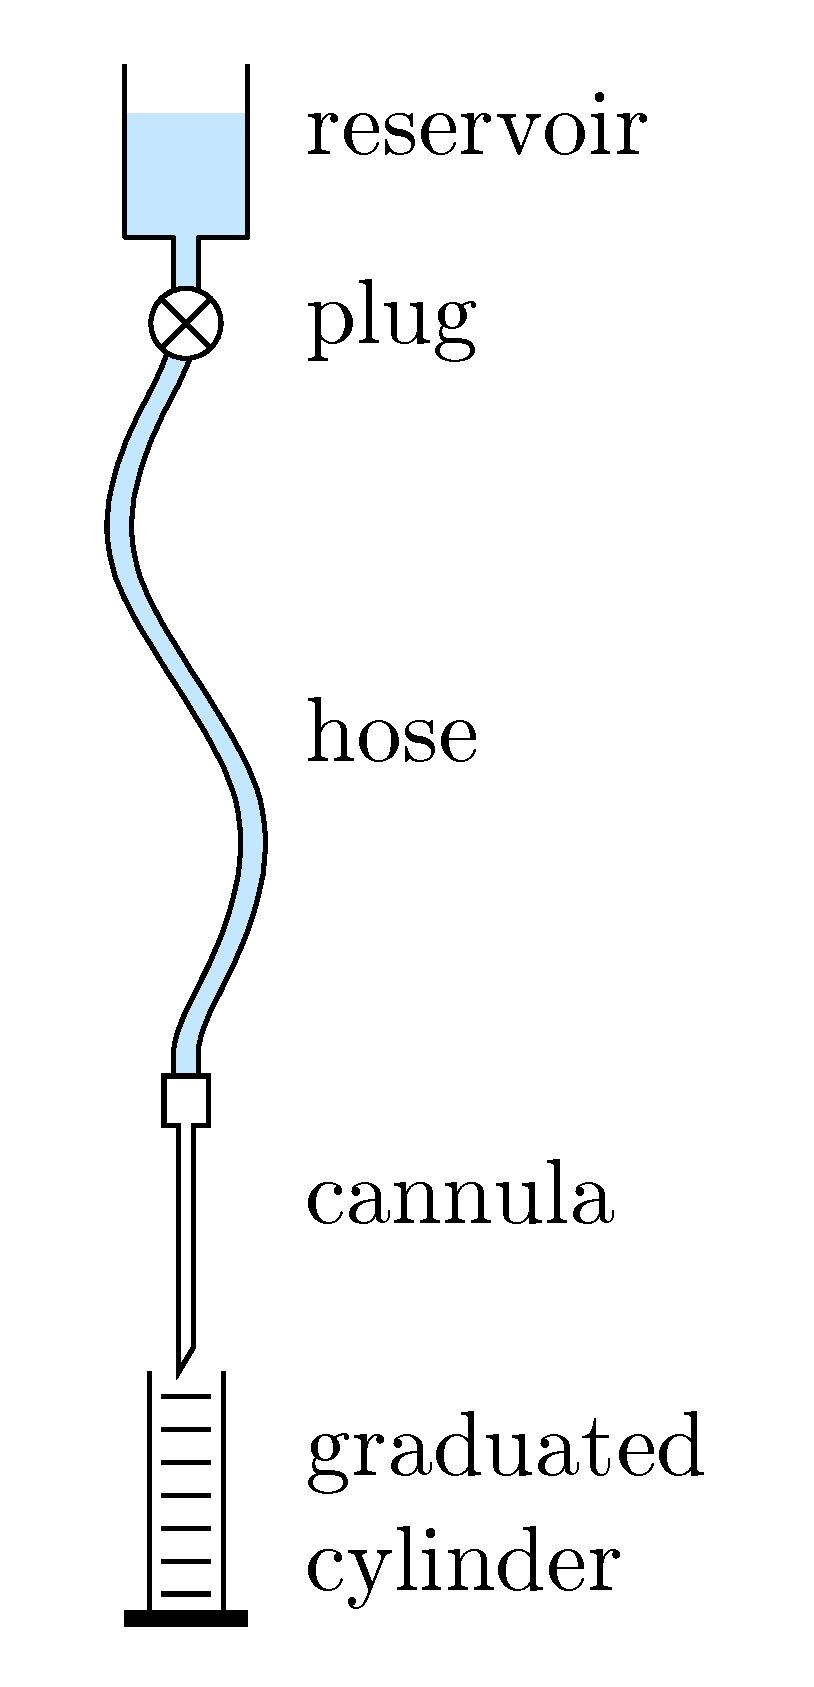
\includegraphics[scale=.25]{Bilder/kanuelen.pdf}
    \caption{capillary viscometer}
    \end{minipage}
    \hspace{5mm}
    \begin{minipage}{.3\textwidth}
    \centering
    \vspace{-.2mm}
    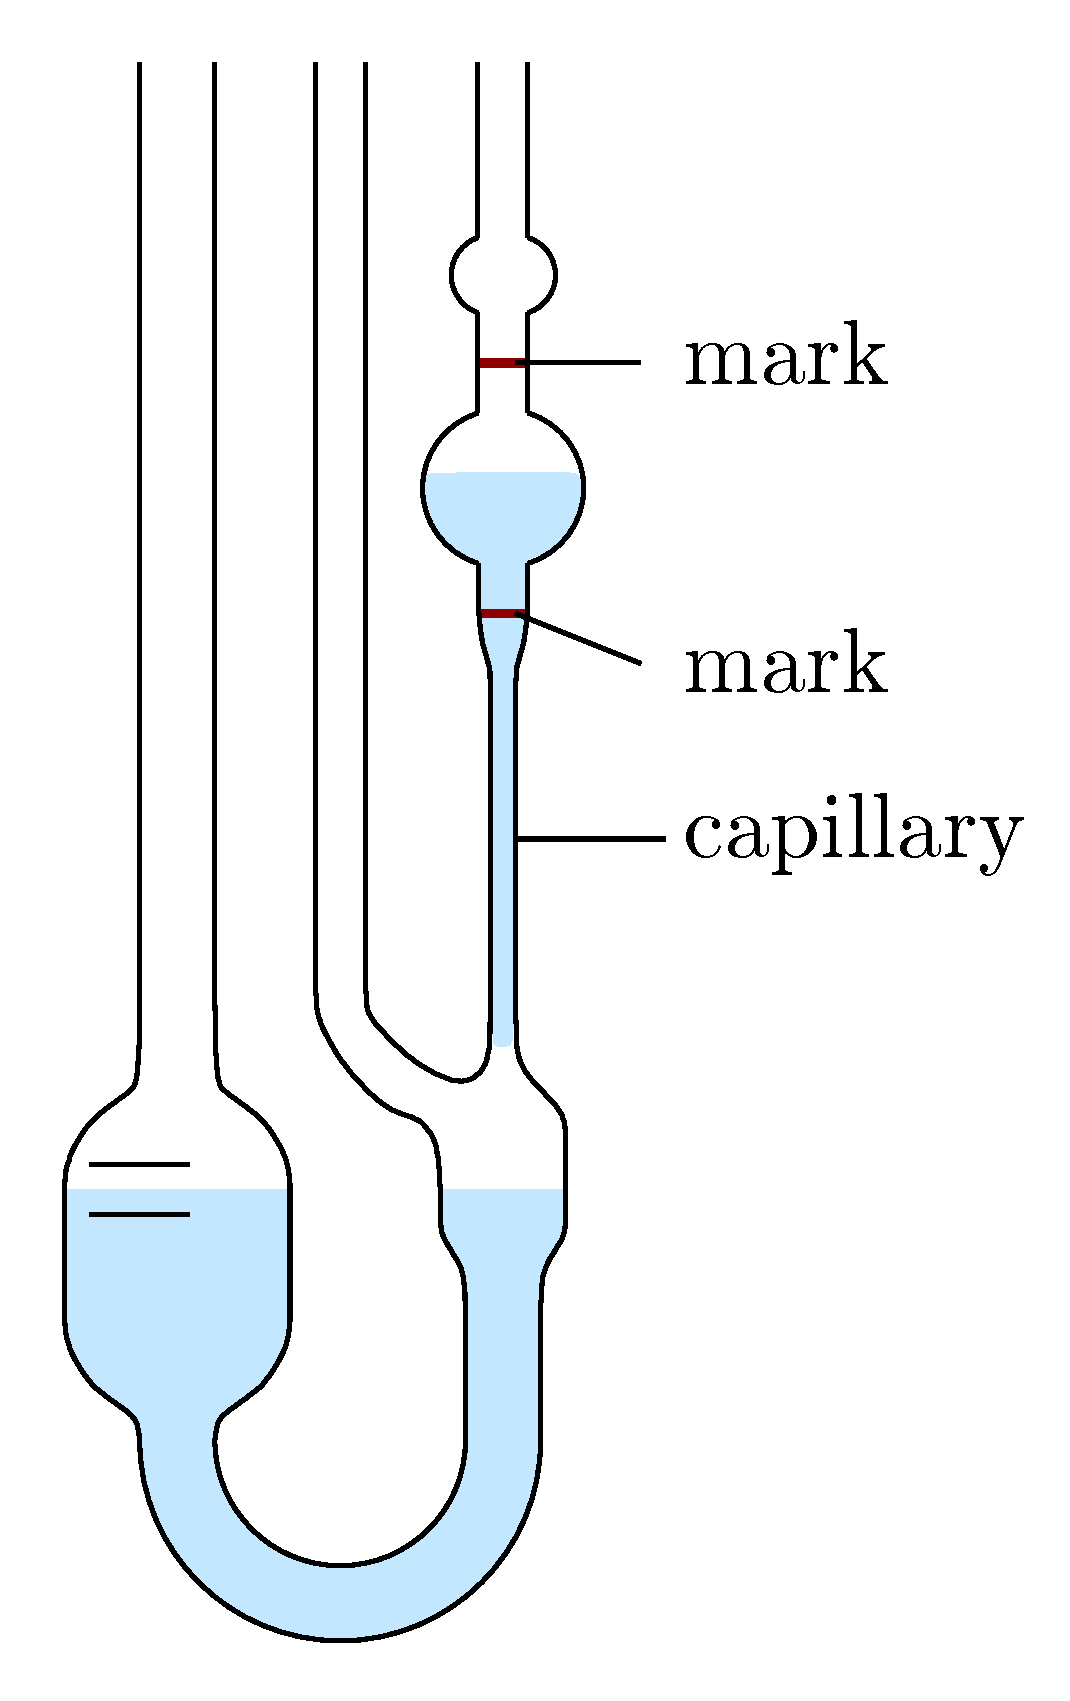
\includegraphics[scale=.25]{Bilder/fancy.pdf}
    \vspace{-.2mm}
    \caption{Ubbelohde viscometer}
    \end{minipage}
\end{figure}